%LLPStartPreview para rodar o pdf com mudancas automaticas


\documentclass{article}
\usepackage{graphicx}
\usepackage{wrapfig}
\usepackage[utf8]{inputenc}
\usepackage[brazil]{babel} % Separacao de silabas em portugues
\usepackage{amsthm} % has proof
\usepackage{listings}

\graphicspath{
    {.} % document root dir
    {img/}
}

\renewcommand\refname{Referências}
\newtheorem{theorem}{Teorema}[section]
\newtheorem{corollary}{Corolário}
\newtheorem{lemma}{Lema}

\title{O problema do carteiro chinês}
\date{}

\begin{document}

\maketitle

\section{As sete pontes de Königsberg}

\begin{wrapfigure}{r}{0.5\textwidth} 
    \centering
    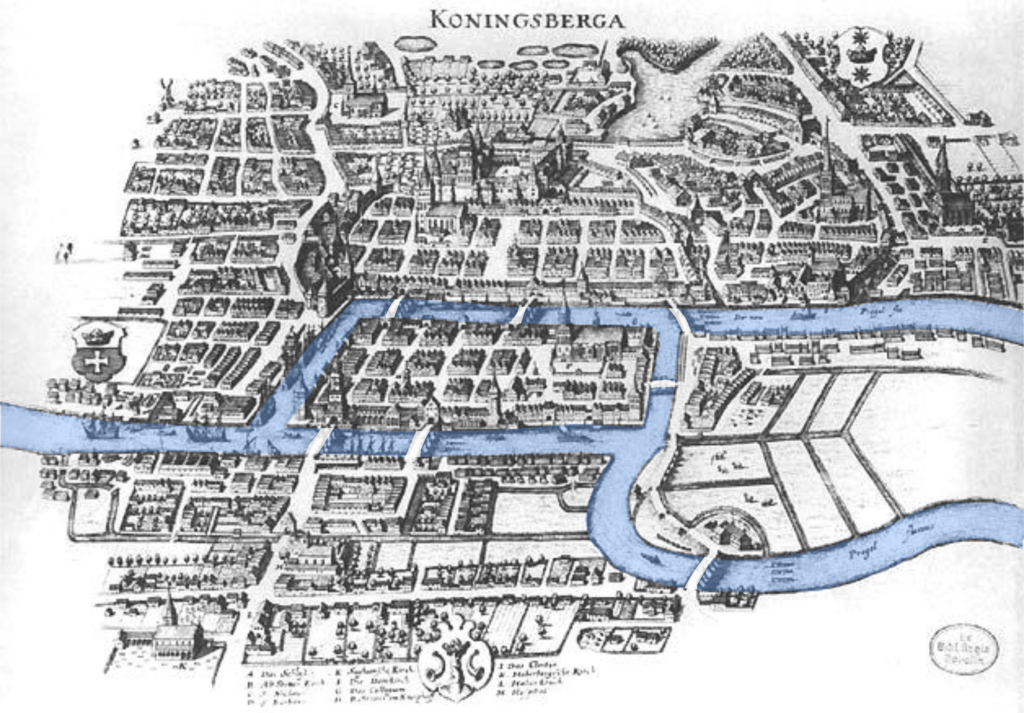
\includegraphics[width=0.5\textwidth]{konigsberg.png}
    \caption{Representação das sete pontes de Königsberg}
\end{wrapfigure}
O problema das sete pontes de Königsberg foi descrito e solucionado pelo matemático Leonhard Euler em 1736, o problema consistia em decidir se seria possível traçar no mapa de Königsberg um trajeto que percorresse cada uma de suas 7 pontes uma única vez, sem repetições.

A importância deste problema é enorme para a área da computação, já que o artigo de Euler publicado sobre ele é considerado o primeiro artigo sobre teoria dos grafos.

Euler resolveu esse problema do seguinte modo: 
Primeiramente, ele identificou cada uma das massas de terra do mapa com as letras A, B, C e D.

Em seguida, ele definiu que um trajeto nesse mapa seria descrito por uma sequência dessas letras: por exemplo, "ACD" indicaria o trajeto que se inicia na massa de terra A, move-se para a massa de terra C, usando uma das pontes, e termina na massa D.

\begin{wrapfigure}{l}{0.5\textwidth} 
    \centering
    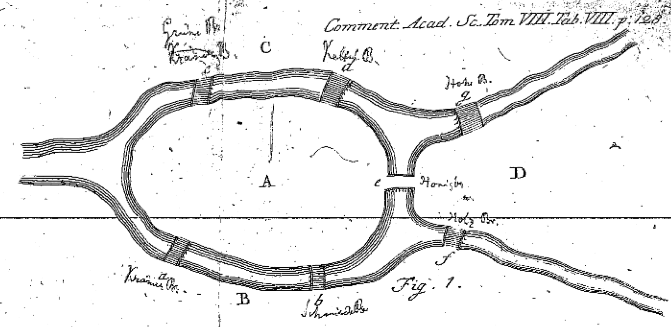
\includegraphics[width=0.5\textwidth]{konigsberg-euler.png}
    \caption{Representação de Euler do problema}
	\label{konigsberg-euler}
\end{wrapfigure}

Euler então começou a definir algumas restrições, assumindo que o problema possuiria alguma solução:

Como o trajeto final deverá passar por todas as 7 pontes exatamente uma vez, isso implica que a sequência de letras que o representa deverá ter tamanho 8.

Além disso, como a massa de terra A possui 5 pontes, necessariamente a letra A aparecerá exatamente 3 vezes na sequência.
A massa B, C e D, no entanto possuem 3 pontes, portanto, suas letras correspondentes deverão aparecer apenas 2 vezes na sequência. 

Chegamos assim a um absurdo, pois inicialmente provamos que a sequência de letras que representa uma solução deveria ter tamanho 8 e depois chegamos que a mesma deveria ter tamanho 9.

Provando assim, por absurdo, que não existe um trajeto como o pedido no enunciado do problema.


A prova do problema em si não foi algo inovador, porém a modelagem de Euler sim, e foi isso que tornou esse problema tão famoso. 
A grande mudança de Euler foi tratar a situação do problema de maneira abstrata, usando letras e linhas, identificando os elementos do problema com letras. 

Essa pequena mudança motivou a criação de uma nova área na matemática, a teoria dos grafos.



Vamos definir como \textbf{passeio} em um grafo uma sequência finita não vazia $P = \{ v_0, a_1, v_2, a_2, \dots, a_k, v_k\}$, cujos termos são alternadamente vértices $v_i$ e arestas $a_j$ e tal que, para todo $i$, $1 \leq i \leq k$, os extremos de $a_i$ são $v_{i-1}$ e $v_i$. 
Os vértices $v_0$ e $v_k$ são a origem e o término de $P$, respectivamente; e os vértices $v_1, v_2, \dots, v_{k-1}$ são chamados vértices internos de P. 

Uma \textbf{trilha} é um passeio sem arestas repetidas. 
Um \textbf{caminho} é um passeio sem vértices repetidos.
Definimos o comprimento de um passeio, denotado por $||P||$, como o número de arestas de $P$.

Um passeio é considerado \textbf{fechado} se sua origem e término são iguais.

Uma trilha fechada, cuja origem e vértices internos são todos distintos, é um \textbf{circuito}.

Devido às contribuições de Euler ao problema descrito, chama-se \textbf{trilha euleriana} como uma trilha que passa por todas arestas de um grafo e \textbf{grafo euleriano} como um grafo que possui uma trilha euleriana fechada.

Euler modelou essa área da cidade como um grafo, representado na figura \ref{konigsberg-graph}, tratando as pontes como arestas e as massas de terra como vértices.
A partir de tal modelagem e das definições feitas, o problema de Königsberg consiste, em definir se o grafo que representa a cidade possui ou não uma trilha euleriana. 


\begin{wrapfigure}{l}{0.25\textwidth}
    \centering
    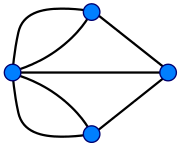
\includegraphics[width=0.25\textwidth]{konigsberg-graph.png}
    \caption{Modelagem de Königsberg como um grafo}
    \label{konigsberg-graph}
\end{wrapfigure}

Apesar de ter recebido grande parte do crédito pelas suas implicações, Euler não provou que qualquer grafo conexo com vértices de grau par era euleriano, essa prova só foi publicada mais de cem anos depois, em 1873, por Carl Hierholzer \cite{hierholzer}, no que se tornou o conhecido Teorema de Euler.


\begin{theorem}[Teorema de Euler ou de Euler-Hierholzer]
    \label{euler}
    Um grafo é euleriano se, e somente se, é conexo e todos seus vértices possuem grau par.
\end{theorem}

Antes de mostrar a prova de tal teorema, primeiramente apresentaremos o seguinte lema:

Seja $\delta(G)$ o grau mínimo de um vértice pertencente a $G$.

\begin{lemma}
	\label{lema}
	Se $G$ é um grafo tal que $\delta(G) \geq 2$, então $G$ possui um caminho fechada.
\end{lemma}

\begin{proof}
	Vamos assumir que um grafo qualquer $G = \{V, A\}$ não possui um caminho fechado. 
	Seja $P$ um caminho de comprimento maximal pertencente a $G$, denominamos $v$ um dos extremos de $P$. 
	Como $P$ é um caminho de comprimento maximal, é impossível, por definição, que $v$ possua uma aresta $vu$ que o ligue a um vértice $u$ não pertencente a $P$.
	
	Como, da premissa, todos vértices possuem grau maior ou igual a 2, isso implica que $v$ possuirá ao menos duas arestas que o ligam à vértices pertencentes a $P$.

	Porém, como $v$ é um vértice extremo de $P$, apenas uma dessas arestas pode pertencer ao caminho $P$. Isso implica que a outra aresta, digamos $vw$, não pertencente a $P$, implica na existência de um caminho fechado.

	Basta tomar o subcaminho entre os vértices $v$ e $w$ pertencente à $P$ juntamente com a aresta $vw$ que teremos um caminho fechado. Chegando assim em uma contradição.

	Demonstra-se assim que $G$ deverá possuir ao menos um caminho fechado dadas as condições do lema.
\end{proof}

Provado tal lema, podemos agora provar o teorema \ref{euler}:

\begin{proof}

Seja $G = \{V, E\}$ o grafo em questão.

Começamos provando que se um grafo é euleriano e conexo então todos seus vértices possuem grau par.

Seja $T$ uma trilha euleriana fechada, cuja existência é garantida já que $G$ é euleriano. Cada vez que um vértice $v$ ocorre em $T$ ela é precedida de uma aresta que liga um vértice qualquer a $v$ e sucedida de outra aresta ligando $v$ a um vértice qualquer. 
Um caso especial é quando o vértice $v$ em questão é a origem (e o término) de $T$: neste caso a aresta que o precede é a última aresta presente em $T$, e a aresta que o sucede é a primeira aresta da trilha.


Agora, provaremos por indução no número de arestas de $G$ que se $G$ for conexo e se todos seus nós possuem grau par, então ele é euleriano.

O caso base da indução é quando não há arestas em $G$. 
O único grafo conexo que respeita tal condição é o grafo que possui apenas um vértice $v$.
Neste exemplo, $\{v\}$ é a trilha euleriana fechada do grafo.

A hipótese de indução é que todo grafo simples, conexo, que possui até $k-1$ arestas e cujos vértices tem grau par é euleriano. 
Seja $G$ um grafo conexo, de vértices de grau par e que possua $k$ arestas.

Como $G$ é conexo, vale que $\delta(G) \geq 1$, mas como todos nós de $G$ têm grau par, podemos afirmar que $\delta(G) \geq 2$. 
Sendo assim, pelo lema \ref{lema}, $G$ deverá possuir um caminho fechado $C$.

Se $C$ possui todas arestas de $G$, então $C$ é uma trilha euleriana fechada do grafo, finalizando a prova.

Do contrário, retira-se de $G$ as arestas pertencentes a $C$, resultando assim em um grafo $G'$. 
Possivelmente $G'$ será desconexo, por isso dizemos que $G'$ será igual a união de $k$ componenetes conexas $G'_1, G'_2, G'_3, \dots, G'_k$ disjuntas entre si.

O grau dos vértices dessas componenentes $G'_i$ deverá ser par, já que ao retirar todas as arestas de uma trilha fechada do grafo $G$ estamos diminuindo os graus de seus vértices em uma quantidade par, mantendo assim a paridade dos graus. Além disso, cada componenete conexa de $G'$ possuirá uma quantidade de arestas menor do que $k$.

Portanto, pela hipótese da indução, cada uma dessas componentes deverá possuir uma trilha euleriana fechada própria. 
Chamaremos de $T_i$ a trilha euleriana fechada da componente $G'_i$.

Segue, assim, o procedimento para a construção de uma trilha euleriana fechada para $G$, que chamaremos de $T$:


Definimos como $CT$ um conjunto de trilhas eulerianas que inicialmente é igual ao conjunto $\{T_1, T_2, \dots, T_k\}$.

Começamos a construção de nossa trilha euleriana fechada a partir de um vértice $v$ qualquer de $C$.

Define-se então uma ordem para $C$ que se inicia no vértice $v$:

\[
	C = \{v, vv_2, v_2, v_2v_3, v_3, \dots, v_n, v_nv\}
\]

Para cada elemento $e$ de $C$ devemos realizar as seguintes verificações:

Começamos adicionando $e$ à trilha euleriana $T$ que estamos construindo.

Se $e$ for um vértice e fizer parte de alguma trilha euleriana $T_i$ pertencente a $CT$, podemos representar $T_i$ como:

\[
	T_i = \{eu_2, u_2, u_2u_3, u_3, \dots, u_k, u_ke, e\}
\]

Basta então adicionarmos a trilha $T_i$ como representada na trilha $T$ e remover do conjunto $CT$ a trilha $T_i$, indicando que ela já foi adicionada à trilha $T$.

Enquanto $e$ ainda pertença a alguma trilha $T_j$ de $CT$, então repetimos o procedimento acima, adicionando $T_j$ à $T$ e removendo a mesma de $CT$.


Ao final desse procedimento, o conjunto $CT$ deverá ser vazio, já que toda trilha $T_i$ possui pelo menos um vértice em $C$. Além disso, toda trilha $T_i$ deverá ter sido adicionada à $T$ uma única vez, já que logo após adicionar uma trilha à $T$ já a removiamos de $CT$, impedindo que ela fosse repetida na trilha euleriana final.

Comprovado o passo da indução, finalizamos a prova do Teorema de Euler.

\end{proof}

\begin{corollary}
    Um grafo possui uma trilha euleriana se, e somente se, é conexo e possui apenas zero ou dois vértices de grau ímpar.
\end{corollary}

\begin{proof}
    Seja $G$ um grafo conexo qualquer. Realizaremos a demonstração para os seguintes casos:
    \begin{enumerate}
        \item $G$ não possui vértices de grau ímpar. Neste caso, $G$ possui, segundo o teorema \ref{euler}, um circuito euleriano, que é um tipo de caminho euleriano.
        
        \item $G$ possui apenas um vértice de grau ímpar. 
			Este caso é impossível de se acontecer, já que a soma do grau de todos vértices deve ser par, impossibilitando assim que apenas um vértice tenha grau ímpar.
        
        \item $G$ possui dois vértices de grau ímpar. 

			Sejam $u$ e $v$ os únicos vértices de $G$ que possuem grau ímpar.
			Adiciona-se uma aresta fictícia ao grafo $G$, a aresta $uv$, fazendo com que tanto $u$ quanto $v$ possuam graus pares. 
			Chamaremos o grafo $G$ acrescido da aresta $uv$ de $G'$.
			Como $u$ e $v$ eram os únicos vértices de grau ímpar de $G$, vale que todos vértices de $G'$ possuirão grau par. 
			Além disso, vale que $G'$ é conexo, pois faz parte da premissa que o grafo original $G$ era conexo.

			Sendo assim, podemos aplicar o teorema \ref{euler}, provando a existência de uma trilha euleriana fechada em $G'$, que chamaremos de $T$.
			Como $T$ é uma trilha euleriana fechada, isso implica que $uv \in T$, e portanto podemos escrever $T$ como:
		
			\[
				T = \{uv, v, ve_1, e_1, e_1e_2, e_2, \dots, e_ku, u\}
			\]

			Deste modo, basta tomar $T' = T - uv$, que teremos uma trilha euleriana válida, usando apenas arestas do grafo original.


        \item $G$ possui três ou mais vértices de grau ímpar. 

			Assuma que existe uma trilha euleriana $T$ para $G$. 
			Neste caso, como pelo menos 3 vértices possuem grau ímpar, necessariamente existirá um vértice $v$ que não é nem o primeiro nem o último vértice de $T$.
			Isso implica que todas aparições de $v$ em $T$ são internas ao caminho, ou seja, toda aparição de $v$ será precedida e sucedida de arestas ligadas a $v$.
			Como estamos tratando de uma trilha euleriana, sabemos que todas arestas adjacentes a $v$ estão presentes em $T$ uma única vez. 
			Mas como todas arestas de $v$ devem aparecer em pares (precedendo e sucedendo $v$), isso implica que o grau de $v$ deverá ser par.
			Contradizendo a premissa.

			Por essa contradição provamos que  $G$ não possuirá trilha euleriana se tiver três ou mais vértices de grau ímpar.
    \end{enumerate}
\end{proof}


Segue agora uma implementação de um algoritmo que encontra o circuito euleriano de um grafo dado que o mesmo possui um circuito euleriano:

 
\lstinputlisting[language=c++]{euler_cycle.cpp}


\section{O problema do Carteiro Chinês}

Com o passar dos anos, a área de teoria dos grafos se desenvolveu muito, tratando dos mais variados tipos de problemas.

Em 1962, mais de 200 anos após Euler descrever sua solução para o problema de Konigsberg, o matemático chinês Meigu Guan publicou um estudo que generalizava ainda mais o problema dos grafos eulerianos. 
Esse problema foi denominado Problema do Carteiro Chinês, ou Problema da Inspeção de Rotas.

A ideia desse problema é encontrar um passeio fechado que visite toda aresta de um grafo conexo pelo menos uma vez. 
A grande diferença aqui é que as arestas podem ser repetidas, ou seja, usadas mais de uma vez no trajeto final.

O nome do problema está relacionado a um problema que carteiros encontram no planejamento de suas rotas: dada uma cidade com várias ruas de diferentes comprimentos e um posto de carteiros, encontrar a menor rota que um carteiro deve percorrer de modo a poder entregar cartas em todas as ruas da cidade e voltar ao posto de carteiros no fim de sua rota.

\begin{wrapfigure}{l}{0.3\textwidth} 
    \centering
    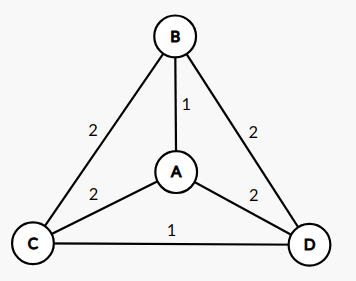
\includegraphics[width=0.3\textwidth]{graph.png}
	\caption{Exemplo de grafo}
	\label{graph}
\end{wrapfigure}

Por exemplo, para a figura \ref{graph}, um passeio fechado de custo ótimo seria: \[ \{A, AB, B, BD, D, DC, C, CA, AD, D, DC, C, CB, B, BA\} \], sendo este um caminho fechado de custo 12.
Neste exemplo foi necessário que as arestas $AB$ (ou $BA$) e $DC$ (ou $CD$) aparecessem duas vezes no passeio, porém nem sempre é necessária esta repetição.

No caso em que o grafo tratado é euleriano, a resposta para o problema do carteiro chinês é justamente a trilha euleriana fechada do grafo.
Nos outros casos, sendo o grafo conexo, o procedimento que seguiremos será similar a realizar a cópia de algumas arestas do grafo de modo a torná-lo euleriano, ou seja, adicionar duplicatas de arestas até que todos os vértices possuam grau par.

Discutiremos nas seções a seguir a solução para o problema em questão com base nas especificidades do grafo do problema:

\subsection{Grafos não direcionados}

Analisaremos o caso em que o problema é modelado a partir de um grafo $G(V, E)$ simples, conexo e com arestas não direcionadas.

A solução se baseia em criar um novo grafo $G'(V', E')$. 
$V'$ é definido como o subconjunto de vértices de $V$ que possuem um grau ímpar em $G$. 
Já $E'$ será definido como o conjunto de arestas entre todo par de vértices de $V'$, dado que uma aresta entre dois vértices $u$ e $v$ quaisquer terá o custo igual ao custo do menor caminho entre $u$ e $v$ no grafo original $G$.

% TODO: Finalizar solução para grafo não direcionado. Fazer exemplo.

\textbf{Solução:} 
\begin{enumerate}
    \item Criar um grafo completo ligando todos vértices $u, v$ que possuirem grau ímpar com arestas de custo igual ao menor caminho entre $u$ e $v$. 
    \item Rodar algoritmo de emparelhamento perfeito de custo mínimo (Húngaro com otimização do Edmonds e Karp, $\mathcal{O}(n^3)$).
\end{enumerate}


\textbf{Observações:}
\begin{itemize}
		\item Pelo ``Lema do aperto de mão'' é garantido que haverá um número par de vértices de grau ímpar.
		\item Essa solução não se aproveita do grafo ser esparso, há outra formulação do Edmonds e Johnson que leva isso em consideração.
		\item Um problema similar é o de cobrir todas arestas com ciclos simples, de modo que o comprimento total dos ciclos é minimizado. Para grafos planares esses problemas são equivalentes.
	\end{itemize}

	\section{Directed CPP}

	O grafo deverá ser fortemente conexo.\\

	\textbf{Solução:}
	\begin{enumerate}
		\item Criar um grafo $P, Q$-bipartido completo. $P$ deve conter todos os vértices do grafo original com excesso de grau de entrada, e $Q$ deve conter todos vértices com excesso de grau de saída. que possuem valores diferentes de grau de entrada e saída. O custo das arestas entre $P$ e $Q$ deverá ser igual ao custo do menor caminho entre os dois vértices que a mesma liga.
		\item Modelar uma rede de fluxo: vértices de $P$ recebem um excesso igual a diferença do grau de entrada pelo grau de saída, vértices de $Q$ recebem uma demanda igual a diferença do grau de saída pelo grau de entrada. 
		\item Rodar um algoritmo de fluxo de custo mínimo. 
	\end{enumerate}

	\textbf{Observações:}
	\begin{itemize}
		\item Modelagem de fluxo com arestas de capacidade unitária, aumentando a velocidade do algoritmo.
	\end{itemize}

	\section{Mixed CPP}

	NP-hard, mesmo se $G$ for planar e se todos $c_{ij}$ forem iguais.

	\section{Windy Postman Problem}

	NP-hard

	Se todo ciclo do grafo tem o mesmo custo em ambos sentidos, transforma a aresta entre $i$ e $j$ de custos $c_{ij}$ e $c_{ji}$ em uma aresta não direcionada com custo $\frac{c_{ij} + c_{ji}}{2}$. Essa transformação reduz o problema de a um CPP não direcionado, que tem solução polinomial, porém para isso é necessário checar se todo ciclo tem o mesmo custo nas duas direções.

	\section{Hierarchical Postman Problem}

	NP-hard 

	Seja $P = \{A_1, A_2, \dots, A_k\}$ uma partição do conjunto de arestas $A$. Determinar um caminho em $G$ de custo mínimo que sai de um vértice $s$ e atinge um vértice $t$, respeitando uma hierarquia das arestas. O caminho só poderá possuir uma aresta pertencente a $A_j$ se o caminho passar anteriormente por todas arestas pertencentes a $A_i$, se $i < j$.


	\section{Anotações}

	\begin{itemize}
		\item Todo mixed CPP pode ser transformado em um WPP.
	\end{itemize}

	\medskip

	\begin{thebibliography}{9}
	\bibitem{konigsberg} 
	Euler, Leonhard
	\textit{Solution problematis ad geometriam situs pertinentis}. 
	Comment. Acad. Sci. U. Petrop 8, 128–40, 1736.

	\bibitem{hierholzer}
	Hierholzer, Carl
	\textit{``Über die Möglichkeit, einen Linienzug ohne Wiederholung und ohne Unterbrechung zu umfahren''}, 
	Mathematische Annalen, 6 (1): 30–32, doi:10.1007/BF01442866, 1873.
	\end{thebibliography}
 
\end{document}

\end{document}
